\section{2020 年 12 月 5 日答疑记录}

\subsection{函数的零点与方程的根}

  求方程的根可以转化为求对应函数图形交点的横坐标, 或求对应函数的零点. 
  一般有如下两种转化方法:
  \begin{align*}
    f(x)=0\text{\ 的根}&\Leftrightarrow 
      \text{$f(x)$ 的图形与 $x$ 轴交点的横坐标};\\
    f(x)+g(x)=0\text{\ 的根}&\Leftrightarrow 
      \text{$f(x)$ 与 $-g(x)$ 的图形交点的横坐标}.
  \end{align*}
  前一种方法可视为后一种方法的特例, 而两种方法在使用时都需要考虑函数的单调性.
  此外还有 (画图更容易理解)
  
  \myemph{零点存在性定理}: 若 $f(x)$ 在 $[a,b]$ 上连续, 且 $f(a)f(b)<0$, 
  则 $f(x)$ 在 $(a,b)$ 上至少有一根. 

\begin{example}\label{exa:201217-1900}
    已知函数 $f(x)= \begin{cases}
        \dfrac2x, & x\geqslant 2,\\
        x^2-3, & x<2,
    \end{cases}$ 若关于 $x$ 的方程 $f(x)=k$ 有三个不等的实根, 求 $k$ 的取值范围.
\end{example}
\begin{solution}
    此题应考虑函数 $y=f(x)$ 与 $y=k$ 的图形的交点恰有三个的情形. 画出两者的图形示意图, 容易知道 $k\in(0,1)$.
    
    \begin{center}
        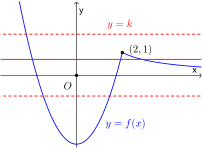
\includegraphics[scale=1]{2020-1214-1900-crop}
    \end{center}
\end{solution}

\begin{example}\label{exa:201214-1905}
    求函数 $f(x)=x^2-\log_{\frac12} x$ 的零点个数.
\end{example}
\begin{solution}
    由 $f(x)=x^2-\log_{\frac12} x=0$ 可得 $x^2=\log_{\frac12} x$, 故设 $g(x)=x^2$, $h(x)=\log_{\frac12} x$, 并考虑两者图形的交点个数. 画图可知, 只有一个交点.
    
    \begin{center}
        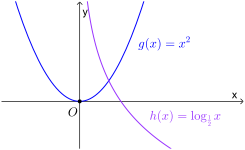
\includegraphics[scale=1]{2020-1214-1910-crop}
    \end{center}
\end{solution}
\begin{remark}
    可以进一步用零点存在性定理来估计例~\ref{exa:201214-1905} 中的 $f(x)$ 的零点所在的大致区间. 因为已经由图知道 $f(x)$ 的零点为正数, 所以只需考虑 $x\in(0,+\infty)$ 的情形. 又因为此时 $\log_{\frac12} x$ 单调递减, 而 $-\log_{\frac12} x$ 单调递增, 所以 $f(x)=x^2-\log_{\frac12} x$ 单调递增. 计算知, $f\biggl(\dfrac12\biggr)=-\dfrac34$, $f(1)=1$, 由零点存在性定理, 零点在区间 $\biggl(\dfrac12,1\biggl)$ 内.
\end{remark}

\begin{example}
    设函数 $f(x)= \begin{cases}
        x, & x<a,\\
        x^2, & x\geqslant a,
    \end{cases}$ 若对于任意实数 $b$, 关于 $x$ 的方程 $f(x)-b=0$ 总有实根, 求 $a$ 的取值范围.
\end{example}
\begin{solution}
    由 $f(x)$ 的表达式可知, 其图形在 $(-\infty,a)$ 上为直线 $y=x$ 的一部分, 在 $[a,+\infty)$ 上为抛物线 $y=x^2$ 的一部分. 而方程 $f(x)-b=0$ 等价于 $f(x)=b$, 则 $a$ 的取值应使得 $y=f(x)$ 与 $y=b$ 的图形总有交点. 画图可知, 仅当 $a\in[0,1]$ 时满足题意.
    
    \begin{center}
        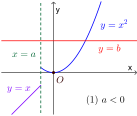
\includegraphics[scale=1]{2020-1214-1920-crop}\qquad
        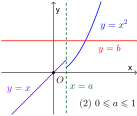
\includegraphics[scale=1]{2020-1214-1930-crop}\qquad
        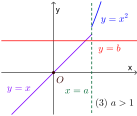
\includegraphics[scale=1]{2020-1214-1940-crop}
    \end{center}
\end{solution}

\begin{example}
    ``$t\geqslant 0$'' 是 ``函数 $f(x)= x^2+tx-t$ 在 $(-\infty,+\infty)$ 内存在零点'' 的什么条件? 
\end{example}
\begin{solution}
    函数 $f(x)= x^2+tx-t$ 在 $(-\infty,+\infty)$ 内存在零点的充要条件是 $\Delta= t^2-4(-t)\geqslant 0$ 即 $t\in(-\infty,-4]\cup [0,+\infty)$, 所以 ``$t\geqslant 0$'' 是 ``函数 $f(x)= x^2+tx-t$ 在 $(-\infty,+\infty)$ 内存在零点'' 的充分不必要条件.
\end{solution}

\subsection{解简单的指数、对数方程或不等式}

解简单的指数、对数方程或不等式, 一般是利用指数、对数的单调性 (参考 ``2020 年 11 月 21 日答疑记录''). 具体来说, 有两种方法.

方法一: 化为同底的指数或对数 (简记为 ``化同底''). 例如, 指数方程 $2^x=4$ 可化为 $2^x=2^2$, 由 $y=2^x$ 单调递增可知, $x=2$. 类似地, $\log_2 x= 2$ 可化为 $\log_2 x= \log_2 4$, 由 $y=\log_2 x$ 单调递增可知, $x=4$. 再如, $2^x>4$ 可化为 $2^x>2^2$, 则 $x>2$; $\log_{0.5} x> 2$ 可化为 $\log_{0.5} x> \log_{0.5} 0.5^2$, 由 $y=\log_{0.5} x$ 单调递减可知, $0<x< 0.25$. 注意, 对数函数有自然定义域, 即真数 (此处的 $x$) 大于零.

方法二: 直接取对数或构造指数式. 此方法涉及指数和对数的运算法则 (参考 ``2020 年 11 月 8 日答疑记录''). 例如, 对方程 $2^x=4$ 两边取以 $2$ 为底的对数, 可得 $\log_2 2^x= \log_2 4$, 即 $x=2$. 类似地, 将 $\log_2 x< 2$ 化为 $2^{\log_2 x}< 2^2$, 可知 $0<x<4$ (注意对数函数的自然定义域). 再如, 由 $2^x>3$ 可得 $x>\log_2 3$ (这个例子用前一个方法来解并不方便). 在这些例子中, 新构造的对数式或指数式的底均应与原式中的相同.

\begin{example}
    解下列不等式: 
    
    (1) $\biggl(\dfrac12\biggr)^x>4$;\qquad
    (2) $\log_3 x> 2$;\qquad
    (3) $3^{x^2+x}>9$;\qquad
    (4) $\log_5 (x^2-4x)\leqslant 1$.
\end{example}
\begin{solution}
    (1) 方法一: 不等式化为 $\biggl(\dfrac12\biggr)^x> \biggl(\dfrac12\biggr)^{-2}$, 所以 $x\in(-\infty,-2)$.
    
    方法二: 不等式化为 $\log_{\frac12}\biggl(\dfrac12\biggr)^x< \log_{\frac12} 4= \log_{\frac12} \biggl(\dfrac12\biggr)^{-2}$, 所以 $x\in(-\infty,-2)$.
    
    (2) 方法一: 不等式化为 $\log_3 x> \log_3 9$, 所以 $x\in(9,+\infty)$.
    
    方法二: 不等式化为 $3^{\log_3 x}> 3^2$, 所以 $x\in(9,+\infty)$.
    
    (3) 方法一: 不等式化为 
    \[3^{x^2+x}>3^2,\quad\text{即}\quad x^2+x>2,\]
    解得 $x\in(-\infty,-2)\cup (1,+\infty)$.
    
    方法二: 不等式化为 $\log_3 3^{x^2+x}>\log_3 9$, 仍可解得 $x\in(-\infty,-2)\cup (1,+\infty)$.
    
    (4) 方法一: 不等式化为 
    \[\log_5 (x^2-4x)\leqslant \log_5 5,\quad\text{即}\quad 0<x^2-4x\leqslant 5,\]
    解得 $x\in[-1,0)\cup (4,5]$.
    
    方法二: 不等式化为 $5^{\log_5 (x^2-4x)}\leqslant 5^1$, 仍可解得 $x\in[-1,0)\cup (4,5]$.
\end{solution}